\documentclass[12pt]{amsart}

\usepackage{latexsym}
\usepackage{amsmath}
\usepackage{amsfonts}
\usepackage{amssymb}
\usepackage{graphicx}

\graphicspath{{images/}}

\newtheorem{theorem}{Theorem}[section]
\newtheorem{lemma}[theorem]{Lemma}
\newtheorem{corollary}[theorem]{Corollary}
\newtheorem{proposition}[theorem]{Proposition}
\newtheorem{noname}[theorem]{}
\newtheorem{sublemma}{}[theorem]
\newtheorem{conjecture}[theorem]{Conjecture}

\theoremstyle{definition}
\newtheorem{definition}[theorem]{Definition}
\newtheorem{example}[theorem]{Example}

\theoremstyle{remark}
\newtheorem{remark}[theorem]{Remark}

\numberwithin{equation}{section}

\newcommand{\bb}[1]{\mathbb{#1}}
\newcommand{\ds}{.3}

\begin{document}

\title{TriColorings of Knots}


\author{Lucas Meyers}
\address{Mathematics Department\\
Louisiana State University\\
Baton Rouge, Louisiana}
\email{lmeye22@lsu.edu}

\date{\today}

\begin{abstract}
  Tricoloring is a knot invariant that differentiates knots
  based on whether or knot their diagram can be colored in a
  certain way with 3 colors. In this paper we introduce knots
  and define Tricolorability in terms of both knot diagrams
  and the knot group. We then briefly mention extensions
  of the notions of tricolorability to arbitrary $n$-coloring.
\end{abstract}

\maketitle
\textbf{TODO}:
\begin{enumerate}
\item Remove \textbf{TODO}
\item Iron out figure/image placement before final edition. Too early
  now. Wait till revision is done.
\end{enumerate}

\section{Introduction}
\label{introduction}

One common pattern we see in mathematics is a concern with how
certain objects fit inside other objects. Knot theory studies this
sort of problem. Given a circle $S^1$ what different ways can we embed
it into $\bb{R}^3$ or $\bb{R}^3$  with an additional point at infinity ($S^3$)?
A typical drawing of a knot can be seen in figure~\ref{fig:figure-eight}.

\begin{figure}
  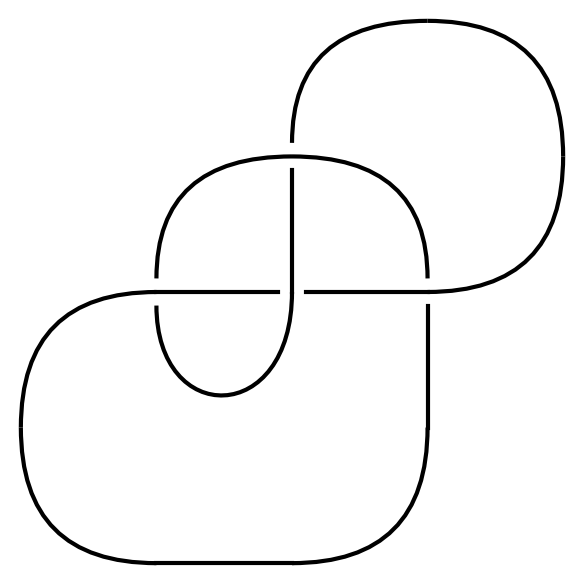
\includegraphics[scale=\ds]{figure-eight}
  \caption{Figure-eight Knot}
  \label{fig:figure-eight}
\end{figure}

Naturally once we begin to consider knots we are also led to consider
how we might tell them apart or rather when they should be the same
at all. Intuitively the knot in figure~\ref{fig:figure-eight} should
be considered the same as in~\ref{fig:figure-eight-t} but should be
different than that of trefoil seen in figure~\ref{fig:trefoil}. In
the next section we will see the definition of a knot, how to define their
equivalence in a sensible way, followed by a method to differentiate them
called tricolorability. Afterwards we will look at an alternative definition
of tricolorability. Then we will introduce notions of how one may consider
coloring knots with more than 3-colors.

\begin{figure}
  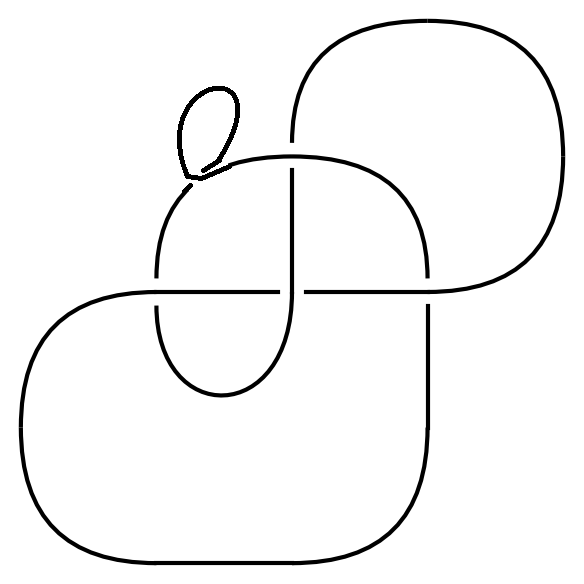
\includegraphics[scale=\ds]{figure-eight-t}
  \caption{Figure-eight with a twist}
  \label{fig:figure-eight-t}
\end{figure}

\section{Diagrams and Coloring}
\label{sec:diagrams-coloring}

In this paper we will follow the conventions of Charles
Livingston~\cite{Livingston}. To begin we give the definition of a knot.

\begin{definition}[Knot]
  A Knot is a simple closed curve in $\bb{R}^3$(or $S^3$).
\end{definition}

Now there are two issues that we need to consider before moving forward.
The first is our notion of equivalence. Unfortunately a homeomorphism from
one knot to another is too weak a notion of equivalence. Instead we will
use an equivalence called ambient isotopy.

\begin{definition}[Ambient Isotopy]
  Two knots $K,J$ are ambient isotopic if there is a homotopy on the ambient
  space $H:S^3\times [0,1]\rightarrow S^3$ if $H(x,0)$ is the identity and the
  image $H(K,1)=J$.
\end{definition}

Second is that we will be considering a subset of knots called tame. A knot
is tame it is ambient isotopic to a piecewise linear knot. An example of
a knot that is not tame is called wild and an example drawing of such can be
seen in figure~\ref{fig:wild}. Wild knots have some more ``pathological''
properties and in order to keep things simple and consistent.

\begin{figure}
  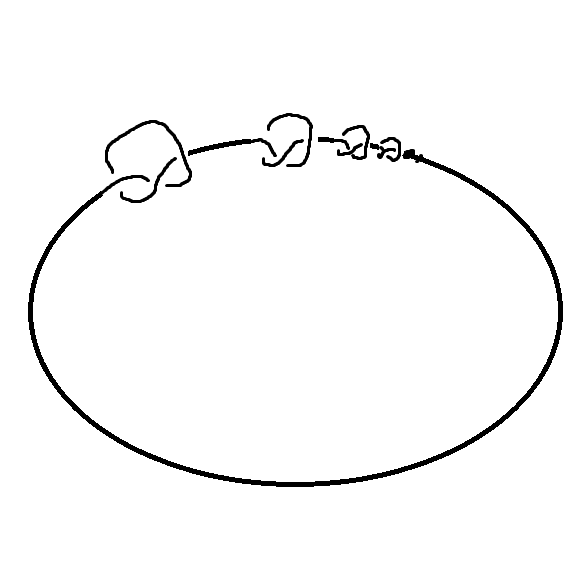
\includegraphics[scale=\ds]{wild}
  \caption{Wild Knot}
  \label{fig:wild}
\end{figure}

When we give the initial definition of  tricolorability we will not work
directly with the curves themselves. Instead we will deal with diagrams
of the knots. All drawings of knots in this paper are examples of diagrams.

\begin{definition}[Diagram]
  A diagram $D$ for a knot $K$ is a projection of $K$ down to a 2-plane
  such that no three points are sent to the same place nor do any two
  points that are kinks in $K$.
\end{definition}

There is a loss of information that occurs when projecting down to a 2-plane
and we recover this by taking any intersection and denoting which strand
goes above and which strand goes below. The segments that make up the
diagram are called arcs.

There is one other unfortunate occurrence
from moving to diagrams. It is that there are infinitely many diagrams
for a given knot. Moreover actually telling whether to diagrams denote
the same knot is extremely difficult although it is decidable and moreover
belongs to NP~\cite{Poonen}.

It turns out that there are three ``moves'' along with planar isotopy
that we can apply to diagrams that will remedy this.

\begin{definition}[Reidmeister Moves]
  The Reidmeister moves are the moves labeled in figure~\ref{fig:reidmeister}.
  We will refer to them as type I, type II, or type III moves respectively.

  \begin{figure}
    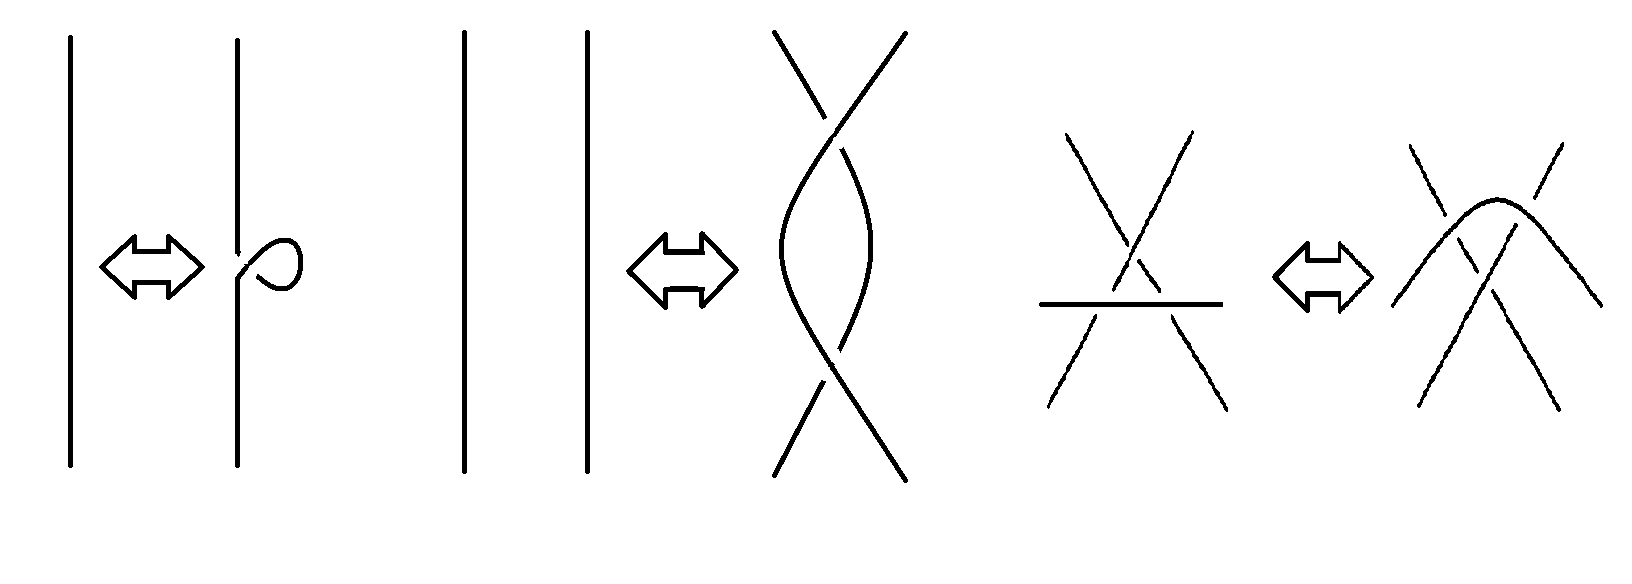
\includegraphics[scale=\ds]{reidmeister}
    \caption{Reidmeister moves}
    \label{fig:reidmeister}
  \end{figure}
\end{definition}

We will use the following theorem about Reidmeister moves without proof.

\begin{theorem}
  Two knots $K$ and $J$ are ambient isotopic if and only if their diagrams
  are related by a finite sequence of Reidmeister moves and planar isotopy.
\end{theorem}

This is where the importance of Reidmeister moves and diagrams becomes apparent
in defining invariants of knots. If we define an invariant on diagrams and show
that it does not change under planar isotopy or the Reidmeister moves then
it will also act as an invariant on knots. This is precisely the method we
will use with our initial definition of tricolorability.

Now there are two knots that we will return to over an over again in this paper
as they are the simplest examples of knots for which tricolorability
differentiates them. The simplest knot is the unknot~\ref{fig:unknot} which
is unique in that it has a diagram with no crossings whatsoever. The
other is the trefoil~\ref{fig:trefoil}.

\begin{figure}
  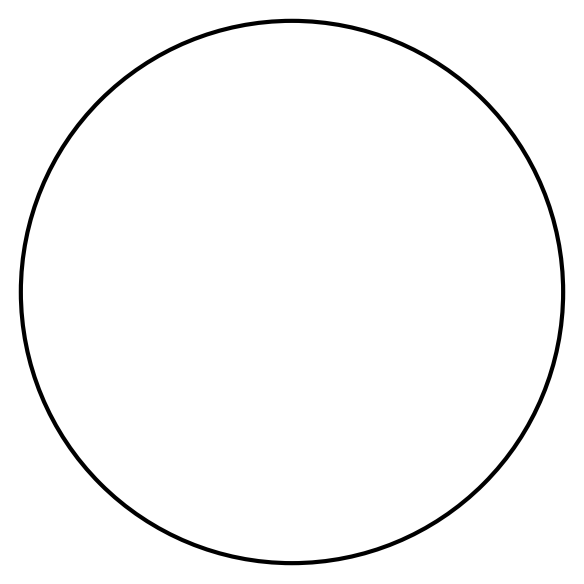
\includegraphics[scale=\ds]{unknot}
  \caption{Unknot}
  \label{fig:unknot}
\end{figure}

\begin{figure}
  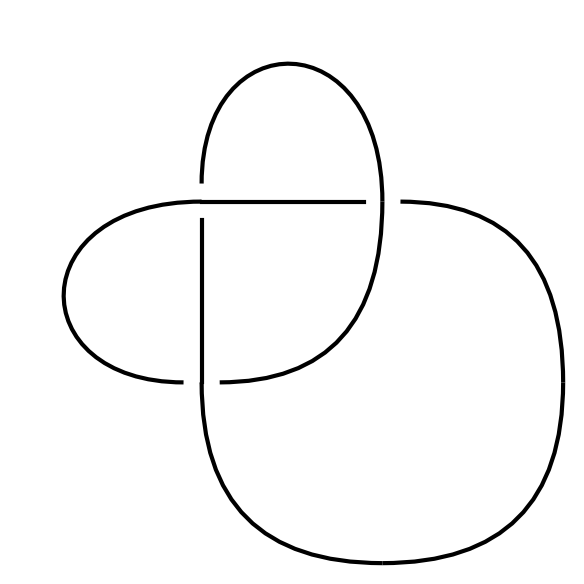
\includegraphics[scale=\ds]{trefoil}
  \caption{Trefoil Knot}
  \label{fig:trefoil}
\end{figure}

With that in mind let us introduce tricolorability.

\begin{definition}
  Let $K$ be a knot with diagram $D$. Then a tricoloring (3-coloring)
  of $K$ is an assignment to each arc one of three colors
  such that at each crossing either all colors or
  only single color color appear. A tricoloring is called nontrivial
  if at least 2 colors are used.
\end{definition}

We will use the colors red, green, and blue as our colors.
Now we must show that tricoloring is in fact an invariant.

\begin{theorem}
  The existence of a non-trivial 3-coloring for some diagram is a
  knot invariant.
\end{theorem}

\begin{proof}
  Let $K$ be a knot with diagram $D$. We must show that given a coloring
  for $D$ that we can color any diagram of $K$. First note that planar isotopy
  does not affect the crossings for $D$ and as such does not change the
  3-colorability.

  Next we will have a series of pictures that demonstrate the possibilities
  for Type I, Type II, and Type III moves respectively.

  For type I we have:
  \begin{figure}
    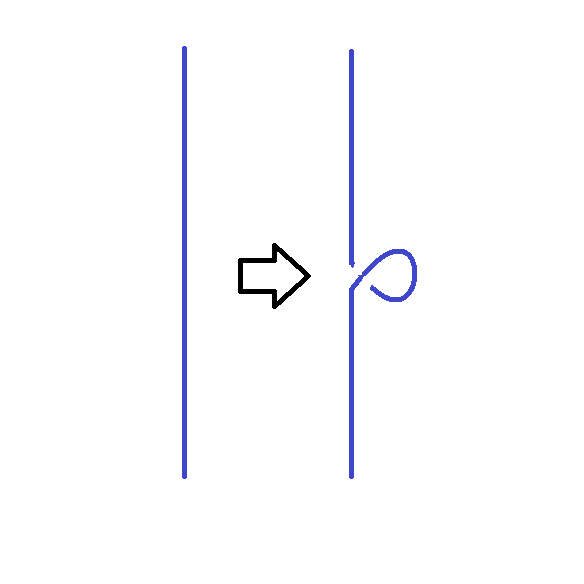
\includegraphics[scale=\ds]{t1-c}
    \caption{Type I}
    \label{fig:t1-c}
  \end{figure}
  
  For type II there are two cases either both strands have the same color
  or they are different.
  \begin{figure}
    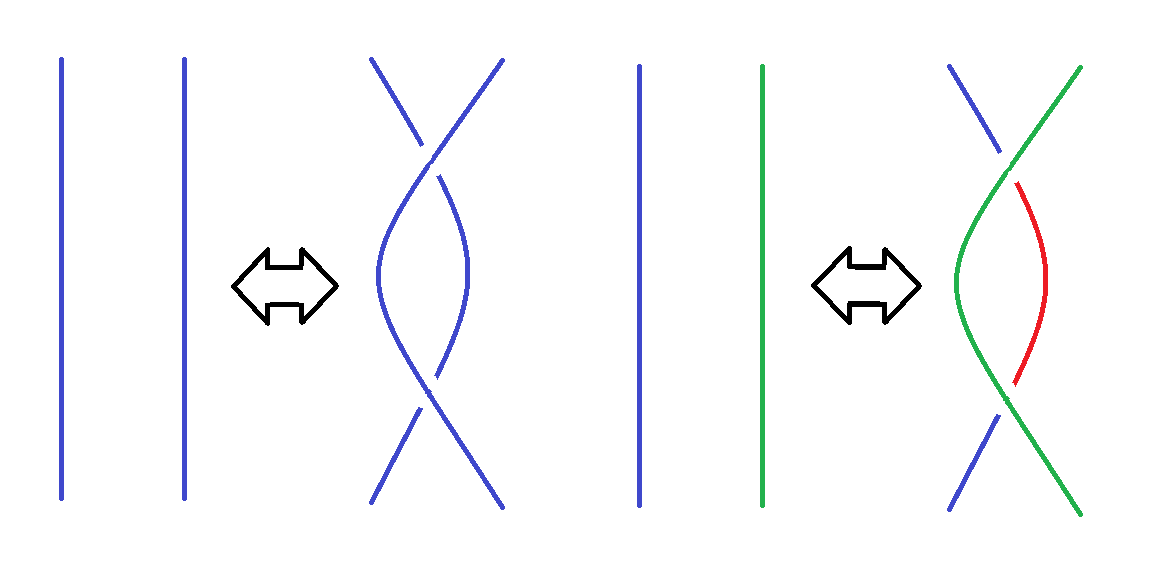
\includegraphics[scale=\ds]{t2-c}
    \caption{Type II}
    \label{fig:t2-c}
  \end{figure}

  Finally for type III moves there are several cases based on
  the colors of the strands entering. We will demonstrate
  three such cases and the rest are similar.
  \begin{figure}
    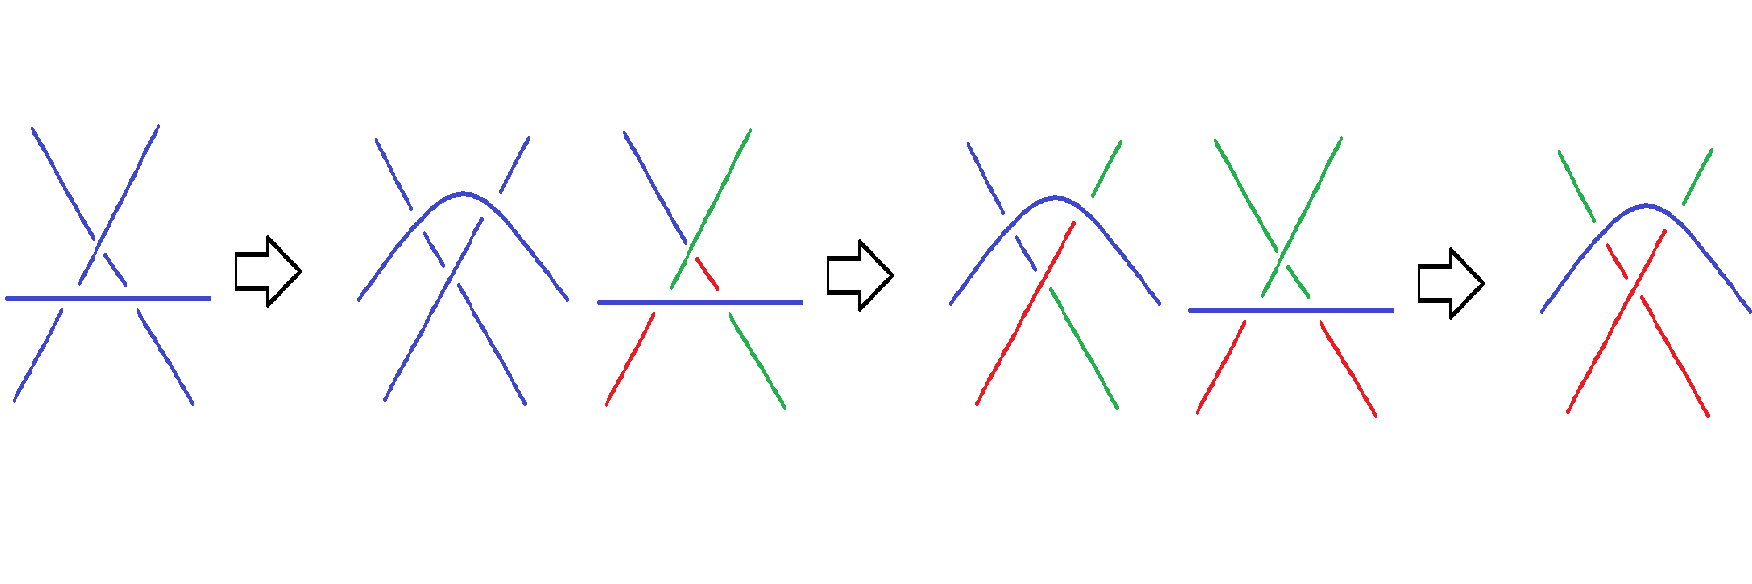
\includegraphics[scale=\ds]{t3-c}
    \caption{Type III}
    \label{fig:t3-c}
  \end{figure}

  Thus if a diagram $D$ for a knot $K$ is has a 3-coloring then
  any diagram for $K$ has a 3-coloring. Therefore 3-colorability
  is a knot invariant.
\end{proof}

An immediate consequence of this is that the unknot and the trefoil
knot are in fact not identical. We can see this because the unknot
is not tricolorable as it only has a single arc. However the
trefoil can be colored as in figure~\ref{fig:trefoil-c}.

\begin{figure}
  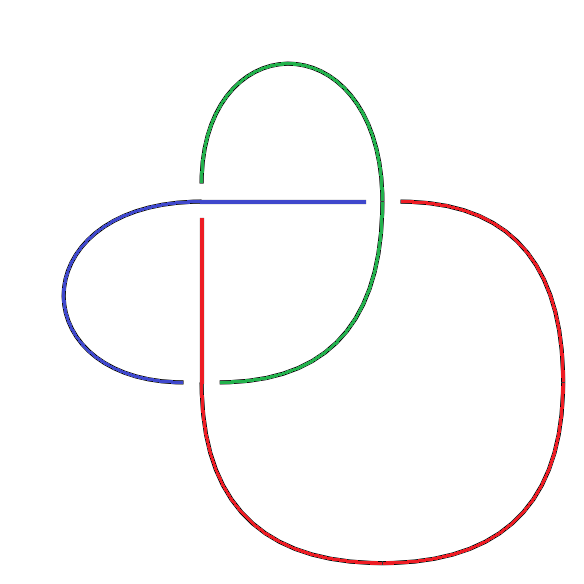
\includegraphics[scale=\ds]{trefoil-c}
  \caption{Colored trefoil}
  \label{fig:trefoil-c}
\end{figure}

\section{The Knot Group}
\label{sec:knot-group-d_6}

The definition of 3-coloring is a perfectly valid definition for a knot
invariant. However it is defined in terms of diagrams and as such
we had to do some extra work with the Reidmeister moves to show that it
was indeed an invariant. Ideally there would be an equivalent definition
of coloring that does not involve diagrams. Then the fact that it is
an invariant would be immediate and it may be possible to better tease
out the topological property that is being captured by 3-coloring.

It turns out that there is a way to define 3-coloring in this manner
and it has to do with a construction called the Knot group. Ones first
instinct to get a group out of a knot might be to take the fundamental
group. However since all knots are copies of $S^1$ the fundamental group
for any knot is $\bb{Z}$. As such we have to take advantage of its
ambient space.

\begin{definition}[Knot Group]
  Let $K$ be a knot. Then the Knot group of $K$ is the fundamental
  group $\pi_1(S^3\setminus K,*)$.
\end{definition}

This definition makes use of the embedding of the knot into $S^3$ and
as such will not be identical for all knots. Naturally we need a way
to calculate the knot group. We can do this using what is called
the Wirtinger presentation~\cite{hatcher}.

\begin{theorem}[Wirtinger]
  Let $K$ be a knot and $D$ a diagram for $K$. Choose an
  orientation for $D$. Then let $x_1,\ldots,x_n$
  denote the arcs of $D$ and for each crossing give a relation
  $r_1\ldots, r_m$ such that $r_i \equiv (x_ix_jx_i^{-1}=x_k)$ where $x_i$ is
  the top arc of the crossing and $x_j$ is the arc underneath approaching
  $x_k$. Then the knot group of $K$ has the presentation
  \[
    \pi_1(S^3\setminus K,*)\cong \langle x_1,\ldots, x_n| \rangle
  \]
\end{theorem}

Now we give a couple of examples.

\begin{example}
  The Knot group of the unknot is
  \[
    \langle x_1 |\rangle \cong \bb{Z}
  \]
  as there are no crossings and only a single arc.
\end{example}

Followed by the trefoil knot.

\begin{example}
  The trefoil knot has three crossings and three arcs. Label it as
  shown in figure~\ref{fig:annotated-trefoil}. Then the Wirtinger presentation
  of the knot group of the trefoil is
  \[
    \langle x_1,x_2,x_3|x_1x_2x_1^{-1}=x_3,x_3x_1x_3^{-1}=x_2,x_2x_3x_2^{-1}=x_1\rangle
  \]
  However the presentation of this group can be simplified to the
  form
  \[
    \langle x_1,x_1| x_1x_2x_1=x_2x_1x_2\rangle
  \]
\end{example}

\begin{figure}
  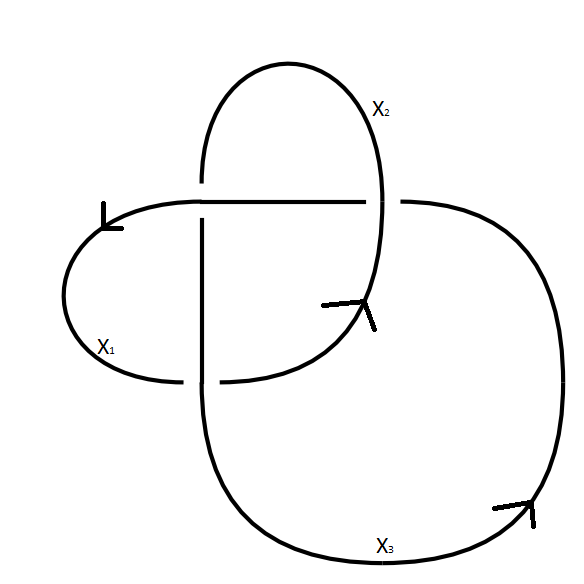
\includegraphics[scale=\ds]{annotated-trefoil}
  \caption{Annotated Trefoil}
  \label{fig:annotated-trefoil}
\end{figure}

The knot group gives us another invariant of knots. Unfortunately
presentations of groups can be rather difficult to work with.
Thus in order to make the problem more tractable we instead look
at homomorphisms from the knot group to finite groups as these
will be determined by where we send generators. This is
how we will redefine coloring in terms of the knot group~\cite{quickfox}.

\begin{definition}[Fox 3-coloring]
  Let $K$ be a knot and $G$ the corresponding knot group. Then a
  Fox 3-coloring of $K$ is a homomorphism $\rho$ from
  $G$ to the symmetries of a triangle $D_6$. We say that
  $\rho$ is a non-trivial coloring if $\rho$ is surjective.

  Thus a knot $K$ is Fox 3-colorable if there exists a nontrivial
  Fox 3-coloring.
\end{definition}

Now a couple of examples using our prior work.

\begin{example}
  The knot group of the unknot is $\bb{Z}$. Since
  $\bb{Z}$ has only a single generator it is not possible to
  create a surjective homomorphism onto $D_6$ as $D_6$ has
  two generators.
\end{example}

\begin{example}
  As we calculated above the knot group for the trefoil is
  \[
    \langle x_1,x_2| x_1x_2x_1=x_2x_1x_2\rangle
  \]
  Similarly we can write a presentation of $D_6$ as
  \[
    \langle r,s| r^3=1, s^2=1,srsr=1\rangle
  \]
  This gives us two non-trivial Fox 3-colorings of the trefoil.
  The first sends $x_1$ to $r$ and $x_2$ to $s$ and the
  other swaps which generator is sent to which generator.
\end{example}

As was implied by the prior examples there is a relation between
Fox 3-coloring and the 3-colorability of knots. In fact it turns
out that they are exactly the same.

\begin{theorem}
  A knot $K$ has a 3-coloring if and only if there is a
  Fox 3-coloring of $K$.
\end{theorem}

A proof of this theorem can be found within~\cite{medwid}. 
The proof that is done relates two notions of coloring using
the Wirtinger presentation to marry the conditions necessary
for the existence of a 3-coloring and the existence of a Fox
3-coloring.

\section{n-coloring}
\label{sec:n-coloring}

So what are the benefits of looking at 3-coloring through
the lens of Fox 3-coloring? As we mentioned before it is
immediately clear that this is a knot invariant where as
when we defined 3-coloring with diagrams. Another benefit
is that it is more readily apparent how we can further
extend Fox 3-coloring than extending 3-coloring. From
the definition of 3-coloring there is some ambiguity that
would need to be sorted out about precisely what rules need
to change. Questions such as ``How many colors are necessary?''
or ``What would make a crossing valid configuration?''.

This is avoided with Fox 3-coloring. The only choice we made
was that we are looking at homomorphisms to $D_6$. We could
very easily have chosen any finite group and gotten the
same nice structure that we had above. The reason that
$D_6$ is the group used for Fox 3-coloring is that it is
the group of symmetries of the triangle. We can
define the Fox $n$-coloring similarly.

\begin{definition}[Fox $n$-coloring]
  Let $G$ be the knot group of a knot $K$. Then
  an $n$-coloring of $K$ is a homomorphism $\rho: G\rightarrow D_{2n}$
  where $\rho$ is called a non-trivial $n$-coloring if $\rho$ is
  surjective.
\end{definition}

We can also extend the notion of coloring that we started
with. However it does take more work. Instead of choosing
the colors that we did when originally defining 3-coloring
we could just as easily have used numbers instead. Then
instead of requiring that each crossing either use all three
colors or all the same it would be equivalent to each
crossing satisfying the equation
\[
  2x-y-z\equiv 0 \mod 3
\]
where the arcs of the crossing are labeled as in figure~\ref{fig:numcolor}.

\begin{figure}
  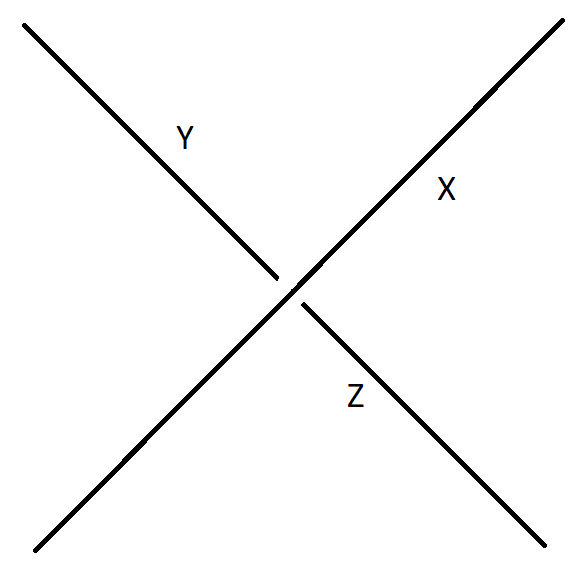
\includegraphics[scale=\ds]{numcolor}
  \caption{Colored Crossing}
  \label{fig:numcolor}
\end{figure}

In this form it is more apparent how we could extend 3-coloring
to arbitrary $n$ by simply replacing the modulus. Going back
to our initial example of a knot, the figure eight knot, we have
an example of a knot that is not 3-colorable but is 5-colorable
as shown in figure~\ref{fig:figure-eight-c}.

\begin{figure}
  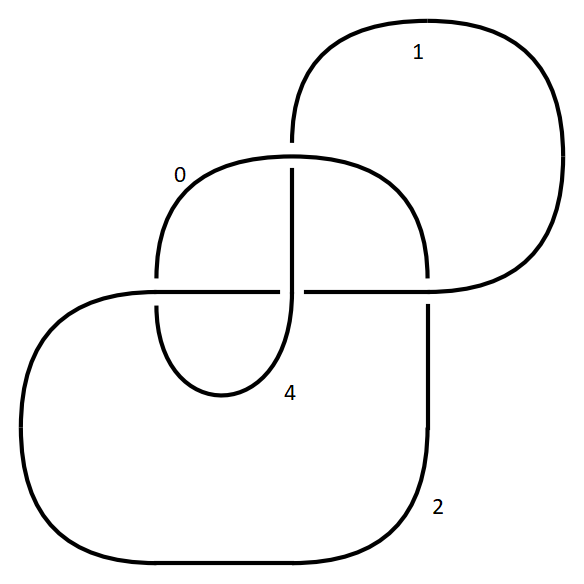
\includegraphics[scale=\ds]{figure-eight-c}
  \caption{Figure-eight 5-coloring}
  \label{fig:figure-eight-c}
\end{figure}

\section*{Acknowledgments}
\begin{thebibliography}{99}

\bibitem{hatcher}  Hatcher, Allen. Algebraic Topology.
  Cambridge University Press, 2017. 
  
\bibitem{Livingston}  Livingston, Charles. Knot Theory.
  Mathematical Association of America, 1996. 
  
\bibitem{medwid}  Medwid, Mark. “Generalized $P$-Colorings of Knots.”
  Bowling Green University, 2014.
  
\bibitem{Poonen}  Poonen, Bjorn. “Undecidable Problems: a Sampler.”
  Interpreting GöDel, pp. 211241., doi:10.1017/cbo9780511756306.015.
  
\bibitem{quickfox}  Fort, M. K., and Ralph H Fox.
  “A Quick Trip Through Knot Theory.” Topology of 3-Manifolds and
  Related Topics, Dover Publications, 2010, pp. 120166.
\end{thebibliography}

\end{document}
